\chapter{Экспериментальный раздел}
\label{cha:research}

В данном разделе будет приведено пример работы программы,
результаты тестирования и сравнение времени работы программы.

\section{Примеры работы}
На рисунке \ref{fig:4.1} приведен пример работы программы.

\begin{figure}[h]
    \centering
    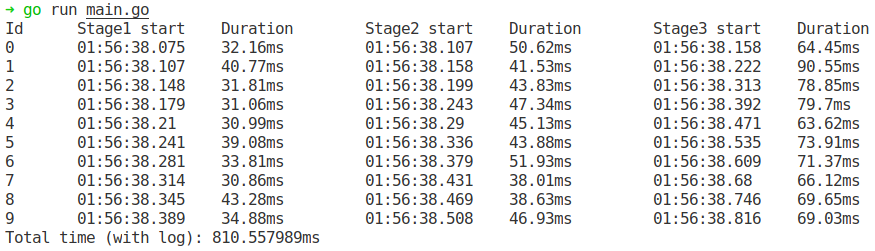
\includegraphics[width=1\textwidth]{5/inc/e1.png}
    \caption{Примеры работы программы}
    \label{fig:4.1}
\end{figure}


\section{Результат тестирования}

На рисунке \ref{fig:4.2} приведен результат тестирования на изображении 1576x890 писель.
(Тестирование в этом случае - это сравнение исходного изображения и результирующего изображения.)

\begin{figure}[h]
    \centering
    
\includegraphics[width=0.42\textwidth]{5/inc/e2.png}
    
\includegraphics[width=0.42\textwidth]{5/inc/e3.png}
    \caption{Результат тестирования}
    \label{fig:4.2}
\end{figure}


% \section{Постановка эксперимента по замеру времени}
\pagebreak
\section{Сравнение времени работы}

Операционная система - Ubuntu 20.04.1 LTS

Процессор - Intel® CoreTM i5-7300HQ CPU @ 2.50GHz × 4 (ЦП 4 ядра 4 потока)

В таблице \ref{tabular:benchmark} приведены замеры времени работы
последовательной параллельной реализации (работает на 3 ядрах),
конвейера (3 стадии, каждый запускается в одном потоке, работают на 3 ядрах)
и параллельного конвейера (3 стадии по три рабочих в каждом, работающих на 3 ядра).
Чтобы быть справедливым, тесты будет использовать до 3-х ядер.


% \def\arraystretch{1.2}
\setlength\tabcolsep{0.2cm}

\begin{table}[h]
    \centering
    \csvreader[tabular=|c|c|c|c|,
        table head=\hline
        \bfseries Кол-во задач
        & \bfseries Последо.
        & \bfseries Конвейер
        & \bfseries Паралл. кон.
        \\\hline,
        late after line=\\\hline]
        {5/inc/benchmark.csv}{}
    { \csvcoli & \csvcolii & \csvcoliii & \csvcoliv}
    \caption{\label{tabular:benchmark} Времени работы (мс)}
\end{table}


% \clearpage
\begin{figure}[!h]
    \centering
    \begin{tikzpicture}
        \begin{axis}[
            scale=1.6,
            axis lines=left,
            xlabel=Количества задач,
            ylabel={Время, мс},
            legend pos=north west,
            xmajorgrids=true,
            ymajorgrids=true,
            ymin=0,
        ]
            \addplot table[x=n,y=t0,col sep=comma] {5/inc/benchmark.csv};
            \addplot table[x=n,y=t1,col sep=comma] {5/inc/benchmark.csv};
            \addplot table[x=n,y=t2,col sep=comma] {5/inc/benchmark.csv};
            \legend{Последовательный (x 3 рабочих), Конвейер (3 стадии), Паралл. конвейер (3стадии x 3рабочих)}
        \end{axis}
    \end{tikzpicture}
    \caption{Зависимость времени работы последовательного реализации, конвейера  и параллельного конвейера от количества задач}
    \label{fig:4.4}
\end{figure}


\section{Вывод}

График показывает, что параллельный конвейер в 2 раз быстрее, чем конвейер,
который использует один поток для каждого этапа (все два используют 3 ядра процессора).
Причина в том, что последний этап требует больше времени для обработки, поэтому предыдущие этапы должны ждать его.
Поскольку конвейер недостаточно длинный и для его реализации требуются дополнительные каналы и передача данных,
поэтому мы не видим здесь разницы между параллельным конвейером и параллельно-последовательной реализацией
(возможно также ОС не равномерно разделила рабочих конвейера на ядра процессора).
